% !TEX program = xelatex
% ============================================================================
%  POSN Computer Qualification — 2D Shapes
%  Topic: รูปสองมิติ (2D Shapes)
% ============================================================================

\documentclass[11pt, aspectratio=169]{beamer}
% ============================================================================
%  POSN Computer Qualification — Shared Beamer Preamble
%  Used by all topic slide decks. Compile with XeLaTeX.
% ============================================================================

% ---------- Thai language & font ----------
\usepackage{iftex}
\usepackage{fontspec}

% XeTeX-specific: enable Thai line breaking
\ifXeTeX
  \XeTeXlinebreaklocale{th}
\fi
% Noto Sans Thai — body text (clean modern sans-serif, handles all Thai)
\setmainfont{Noto Sans Thai}[
  UprightFont = Noto Sans Thai Light,
  BoldFont    = Noto Sans Thai Medium,
  Scale       = 0.9
]
\setsansfont{Noto Sans Thai}[
  UprightFont = Noto Sans Thai Light,
  BoldFont    = Noto Sans Thai Medium,
  Scale       = 0.9
]

% Noto Sans Thai — clean modern sans-serif for structural elements
\newfontfamily\headingfont{Noto Sans Thai}[
  UprightFont = Noto Sans Thai Medium,
  BoldFont    = Noto Sans Thai Bold,
  Scale       = 0.9
]

% --- Heading font for structural elements ---
\setbeamerfont{title}{family=\headingfont, series=\bfseries, size=\huge}
\setbeamerfont{subtitle}{family=\headingfont, series=\mdseries}
\setbeamerfont{author}{family=\headingfont, series=\mdseries}

% --- Custom Title Page ---
\defbeamertemplate{title page}{custom}[1][]{%
  \centering
  \vspace*{2cm}
  % Title — in white
  {\usebeamerfont{title}\color{white}\inserttitle\par}
  \vspace{0.6cm}
  % Subtitle — in white
  {\usebeamerfont{subtitle}\color{white}\insertsubtitle\par}
  \vspace{2.5cm}
  % Author — blue filled rounded box, white text
  \begin{center}
    \begin{tcolorbox}[arc=3mm, colback=boxBlue, colframe=boxBlue!80,
                      width=0.42\textwidth, halign=center,
                      left=1.5em, right=1.5em, top=0.8em, bottom=0.8em,
                      boxrule=1.5pt, coltext=white]
      \usebeamerfont{author}\insertauthor
    \end{tcolorbox}
  \end{center}
}
\setbeamertemplate{title page}[custom]
\setbeamerfont{frametitle}{family=\headingfont, series=\bfseries}
\setbeamerfont{section in toc}{family=\headingfont}
\setbeamerfont{page number in head/foot}{family=\headingfont}
\setbeamerfont{section title}{family=\headingfont, series=\bfseries}
\setbeamerfont{subsection title}{family=\headingfont}

% Monospace font (for code/verbatim)
\setmonofont{Latin Modern Mono}[Scale=0.9]

% ---------- Math ----------
\usepackage{amsmath, amssymb}

% ---------- Graphics ----------
\usepackage{graphicx}
\usepackage{tikz}

% ---------- String parsing (for section headers) ----------
\usepackage{xstring}

% ---------- Colored boxes ----------
\usepackage[skins, breakable, xparse]{tcolorbox}
% Note: we do NOT load the 'most' option — it predefines example/solution environments
% that would conflict with our custom boxes.

% --- Color definitions ---
\definecolor{boxBlue}{RGB}{41, 128, 185}
\definecolor{boxGreen}{RGB}{39, 174, 96}
\definecolor{boxOrange}{RGB}{230, 126, 34}
\definecolor{boxPurple}{RGB}{142, 68, 173}
\definecolor{boxBlueBg}{RGB}{235, 245, 255}
\definecolor{boxGreenBg}{RGB}{235, 255, 240}
\definecolor{boxOrangeBg}{RGB}{255, 245, 235}
\definecolor{boxPurpleBg}{RGB}{248, 240, 255}

% --- Explanation box (blue) — for definitions, concepts, notes ---
\newtcolorbox{explanation}[1][]{
  enhanced,
  breakable,
  arc         = 2mm,
  colback     = boxBlueBg,
  colframe    = boxBlue!50,
  title       = #1,
  fonttitle   = \bfseries\color{white},
  coltitle    = white,
  colbacktitle= boxBlue,
  attach boxed title to top left = {yshift=-2mm, xshift=2mm},
  boxed title style = {arc=2mm, size=small},
  before skip = 8pt,
  after skip  = 8pt
}

% --- Example box (green) — for worked examples ---
\newtcolorbox{exambox}[1][]{
  enhanced,
  breakable,
  arc         = 2mm,
  colback     = boxGreenBg,
  colframe    = boxGreen!50,
  title       = #1,
  fonttitle   = \bfseries\color{white},
  coltitle    = white,
  colbacktitle= boxGreen,
  attach boxed title to top left = {yshift=-2mm, xshift=2mm},
  boxed title style = {arc=2mm, size=small},
  before skip = 8pt,
  after skip  = 8pt
}

% --- Solution box (orange) — for solutions and answers ---
\newtcolorbox{solbox}[1][]{
  enhanced,
  breakable,
  arc         = 2mm,
  colback     = boxOrangeBg,
  colframe    = boxOrange!50,
  title       = #1,
  fonttitle   = \bfseries\color{white},
  coltitle    = white,
  colbacktitle= boxOrange,
  attach boxed title to top left = {yshift=-2mm, xshift=2mm},
  boxed title style = {arc=2mm, size=small},
  before skip = 8pt,
  after skip  = 8pt
}

% --- Intuition box (purple) — for plain-language explanations, analogies ---
\newtcolorbox{intuition}[1][]{
  enhanced,
  breakable,
  arc         = 2mm,
  colback     = boxPurpleBg,
  colframe    = boxPurple!50,
  title       = #1,
  fonttitle   = \bfseries\color{white},
  coltitle    = white,
  colbacktitle= boxPurple,
  attach boxed title to top left = {yshift=-2mm, xshift=2mm},
  boxed title style = {arc=2mm, size=small},
  before skip = 8pt,
  after skip  = 8pt
}

% ---------- Beamer theme ----------
\usetheme{Madrid}
\usecolortheme{default}

% --- Custom beamer colors (blue accent matching explanation boxes) ---
\setbeamercolor{structure}{fg=boxBlue}
\setbeamercolor{palette primary}{fg=white, bg=boxBlue}
\setbeamercolor{palette secondary}{fg=white, bg=boxBlue!80}
\setbeamercolor{palette tertiary}{fg=white, bg=boxBlue!60}
\setbeamercolor{block title}{fg=white, bg=boxBlue}
\setbeamercolor{block body}{fg=black, bg=boxBlueBg}

% Remove navigation symbols for clean look
\setbeamertemplate{navigation symbols}{}

% Note: Frame title prefix removed — \addtobeamertemplate conflicts with beamer internals

% --- Outline (Table of Contents) styling ---
\setbeamerfont{section in toc}{family=\headingfont, series=\mdseries}
\setbeamerfont{subsection in toc}{family=\headingfont, series=\mdseries}
\setbeamertemplate{section in toc}{%
  \leavevmode\leftskip=1.5em
  \textcolor{boxBlue}{\textbf{\large\inserttocsectionnumber.}}%
  \quad\inserttocsection\par
  \vspace{0.2em}
}
\setbeamertemplate{subsection in toc}{%
  \leavevmode\leftskip=4em
  \textcolor{boxBlue!60}{\small$\bullet$}%
  \quad\inserttocsubsection\par
  \vspace{0.1em}
}

% Section header slides — Thai in white, English in smaller light blue below
\AtBeginSection{
  \begin{frame}[plain]{}
    \vspace*{2cm}
    \begin{beamercolorbox}[sep=12pt, center, rounded=true, shadow=true]{palette primary}
      \IfSubStr{\secname}{(}{%
        \StrBefore{\secname}{(}[\sectionthai]%
        \StrBetween[1,1]{\secname}{(}{)}[\sectioneng]%
        \begin{tabular}{@{}c@{}}
          {\usebeamerfont{title}\sectionthai} \\[0.2em]
          {\usebeamerfont{subtitle}\color{boxBlue!60}\sectioneng}
        \end{tabular}%
      }{%
        {\usebeamerfont{title}\secname\par}%
      }
    \end{beamercolorbox}
    \vfill
  \end{frame}
}

% Subsection header slides — smaller, centered
\AtBeginSubsection{
  \begin{frame}[plain]{}
    \vfill
    \centering
    {\usebeamerfont{section title}\insertsubsectionhead\par}
    \vfill
  \end{frame}
}

% Minimal footer: page number only, right-aligned
\setbeamertemplate{footline}{
  \hfill\usebeamerfont{page number in head/foot}\insertframenumber{} / \inserttotalframenumber\hspace*{1em}\vspace*{0.5ex}
}

% ---------- Spacing & readability ----------
\linespread{1.2}

% ---------- Useful commands ----------

% Highlight important text in blue
\newcommand{\highlight}[1]{\textcolor{boxBlue}{\textbf{#1}}}

% Math set notation helpers
\newcommand{\R}{\mathbb{R}}
\newcommand{\N}{\mathbb{N}}
\newcommand{\Z}{\mathbb{Z}}
\newcommand{\Q}{\mathbb{Q}}

% ============================================================================
%  End of preamble
% ============================================================================


\title[รูปสองมิติ]{รูปสองมิติ}
\subtitle{2D Shapes — รูปหลายเหลี่ยม, รูปนูน/เว้า, พื้นที่, เส้นรอบรูป}
\author[None W. (Yuan)]{None W. (Yuan)}
\date{}

\begin{document}

\begin{frame}[plain]\titlepage\end{frame}
\begin{frame}{สารบัญ (Outline)}\tableofcontents\end{frame}

\begin{frame}{ก่อนเรียน (Prerequisites)}
  \begin{explanation}[สิ่งที่ควรรู้ก่อนเรียน]
    \begin{itemize}
      \item \textbf{มุม} — ชนิดของมุม, มุมประกอบ, มุมภายใน
      \item \textbf{สามเหลี่ยม} — ชนิด, ผลรวมมุมภายใน $= 180^\circ$, พื้นที่ $\frac{1}{2}bh$
      \item \textbf{วงกลม} — ส่วนประกอบ, เส้นรอบวง $2\pi r$, พื้นที่ $\pi r^2$
      \item \textbf{สมการ} — การแก้สมการเชิงเส้น
    \end{itemize}
  \end{explanation}

  \begin{intuition}[รูปสองมิติคืออะไร?]
    \textbf{รูปสองมิติ} คือรูปเรขาคณิตที่อยู่บนระนาบ — มีเฉพาะความกว้างและความยาว ไม่มีความลึก
    เช่น สามเหลี่ยม, สี่เหลี่ยม, วงกลม, ห้าเหลี่ยม
  \end{intuition}
\end{frame}

% ===========================================================================
%  SECTION 1: รูปหลายเหลี่ยม
% ===========================================================================
\section{รูปหลายเหลี่ยม (Polygons)}

\begin{frame}{รูปหลายเหลี่ยมคืออะไร?}
  \begin{explanation}[นิยาม]
    \textbf{รูปหลายเหลี่ยม (Polygon)} คือรูปปิดบนระนาบที่ประกอบด้วยส่วนของเส้นตรง (\textbf{ด้าน})
    มาต่อกัน โดยด้านที่อยู่ติดกันบรรจบกันที่ \textbf{จุดยอด}
  \end{explanation}

  \begin{columns}[T]
    \column{0.45\textwidth}
      \begin{center}
        \begin{tikzpicture}[scale=1.1]
          % Pentagon
          \draw[thick, fill=boxBlue!10] (0,0) -- (1.2,0) -- (1.6,1.2) -- (0.6,1.9) -- (-0.4,1.0) -- cycle;
          \foreach \p in {(0,0),(1.2,0),(1.6,1.2),(0.6,1.9),(-0.4,1.0)}
            \fill \p circle (1.2pt);
          \node at (0.6,1.0) {\textbf{รูปห้าเหลี่ยม}};
          \node at (0.6,-0.4) {5 ด้าน, 5 จุดยอด};
        \end{tikzpicture}
      \end{center}

    \column{0.55\textwidth}
      \begin{explanation}
        \begin{itemize}
          \item 3 ด้าน — \textbf{สามเหลี่ยม} (Triangle)
          \item 4 ด้าน — \textbf{สี่เหลี่ยม} (Quadrilateral)
          \item 5 ด้าน — \textbf{ห้าเหลี่ยม} (Pentagon)
          \item 6 ด้าน — \textbf{หกเหลี่ยม} (Hexagon)
          \item $n$ ด้าน — \textbf{$n$ เหลี่ยม} ($n$-gon)
        \end{itemize}
      \end{explanation}
  \end{columns}
\end{frame}

\begin{frame}{รูปหลายเหลี่ยมนูนและรูปหลายเหลี่ยมเว้า}
  \begin{columns}[T]
    \column{0.5\textwidth}
      \centering
      \textbf{รูปหลายเหลี่ยมนูน (Convex)}

      \medskip
      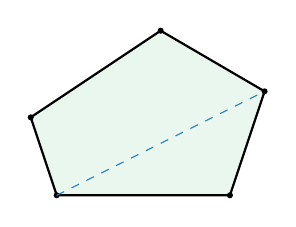
\begin{tikzpicture}[scale=1.1]
        \draw[thick, fill=boxGreen!10] (0,0) -- (2,0) -- (2.4,1.2) -- (1.2,1.9) -- (-0.3,0.9) -- cycle;
        \foreach \p in {(0,0),(2,0),(2.4,1.2),(1.2,1.9),(-0.3,0.9)}
          \fill \p circle (1pt);
        % diagonal inside
        \draw[boxBlue, dashed] (0,0) -- (2.4,1.2);
      \end{tikzpicture}

      \begin{itemize}
        \item มุมภายใน \textbf{ทุกมุม} $< 180^\circ$
        \item เส้นทแยงมุม \textbf{ทุกเส้น} อยู่ภายใน
        \item จุดต่อจุดใด ๆ — ส่วนของเส้นตรงอยู่ภายในรูป
      \end{itemize}

    \column{0.5\textwidth}
      \centering
      \textbf{รูปหลายเหลี่ยมเว้า (Concave)}

      \medskip
      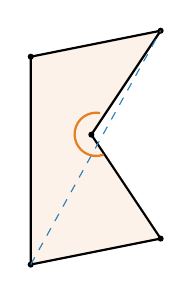
\begin{tikzpicture}[scale=1.1]
        % Arrowhead/dart shape (concave quadrilateral)
        \draw[thick, fill=boxOrange!10] (0,0) -- (1.5,0.3) -- (0.7,1.5) -- (1.5,2.7) -- (0,2.4) -- cycle;
        \foreach \p in {(0,0),(1.5,0.3),(0.7,1.5),(1.5,2.7),(0,2.4)}
          \fill \p circle (1pt);
        % diagonal partly outside
        \draw[boxBlue, dashed] (0,0) -- (1.5,2.7);
        % Mark the reflex angle
        \draw[boxOrange, thick] (0.8,1.75) arc (80:290:0.25);
      \end{tikzpicture}

      \begin{itemize}
        \item มีมุมภายใน \textbf{อย่างน้อย 1 มุม} $> 180^\circ$ (มุมกลับ)
        \item มีเส้นทแยงมุมบางเส้น \textbf{อยู่นอก} รูป
      \end{itemize}
  \end{columns}
\end{frame}

\begin{frame}{รูปหลายเหลี่ยมปกติ (Regular Polygon)}
  \begin{explanation}[นิยาม]
    \textbf{รูปหลายเหลี่ยมปกติ} คือรูปหลายเหลี่ยมนูนที่มี \highlight{ด้านเท่ากันทุกด้าน}
    และ \highlight{มุมเท่ากันทุกมุม}
  \end{explanation}

  \begin{center}
    \begin{tikzpicture}[scale=1.5]
      % Equilateral triangle
      \draw[thick, fill=boxBlue!8] (0,0) -- (1.4,0) -- (0.7,1.212) -- cycle;
      \node at (0.7,-0.3) {สามเหลี่ยมด้านเท่า};

      % Square
      \draw[thick, fill=boxGreen!8] (2.2,0) rectangle (3.6,1.4);
      \node at (2.9,-0.3) {สี่เหลี่ยมจัตุรัส};

      % Regular pentagon
      \draw[thick, fill=boxOrange!8] (4.5,0.3) -- (5.15,0.9) -- (4.85,1.55) -- (4.15,1.55) -- (3.85,0.9) -- cycle;
      \node at (4.5,-0.3) {ห้าเหลี่ยมปกติ};

      % Regular hexagon
      \draw[thick, fill=boxPurple!8] (6.4,0) -- (6.95,0) -- (7.25,0.5) -- (6.95,1) -- (6.4,1) -- (6.1,0.5) -- cycle;
      \node at (6.65,-0.3) {หกเหลี่ยมปกติ};
    \end{tikzpicture}
  \end{center}

  \begin{exambox}[หมายเหตุ]
    สามเหลี่ยมด้านเท่าเป็นรูปหลายเหลี่ยมปกติที่มีจำนวนด้านน้อยที่สุด
  \end{exambox}
\end{frame}

\begin{frame}{จำนวนเส้นทแยงมุม}
  \begin{explanation}[สูตร]
    ในรูป $n$ เหลี่ยมนูน จำนวนเส้นทแยงมุม $= \dfrac{n(n-3)}{2}$
  \end{explanation}

  \begin{columns}[T]
    \column{0.45\textwidth}
      \centering
      \medskip\medskip
      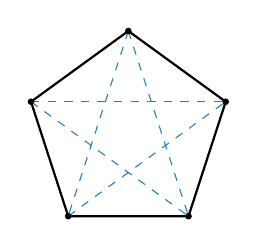
\begin{tikzpicture}[scale=1.0]
        % Pentagon with all diagonals
        \coordinate (A) at (90:1.3);
        \coordinate (B) at (162:1.3);
        \coordinate (C) at (234:1.3);
        \coordinate (D) at (306:1.3);
        \coordinate (E) at (18:1.3);

        \draw[thick] (A) -- (B) -- (C) -- (D) -- (E) -- cycle;
        \draw[boxBlue, dashed] (A) -- (C);
        \draw[boxBlue, dashed] (A) -- (D);
        \draw[boxBlue, dashed] (B) -- (D);
        \draw[boxBlue, dashed] (B) -- (E);
        \draw[boxBlue, dashed] (C) -- (E);

        \foreach \p in {A,B,C,D,E}
          \fill (\p) circle (1.2pt);
      \end{tikzpicture}

    \column{0.55\textwidth}
      \begin{exambox}[ตัวอย่าง]
        \begin{itemize}
          \item $n=3$ (สามเหลี่ยม): $\frac{3(0)}{2} = 0$
          \item $n=4$ (สี่เหลี่ยม): $\frac{4(1)}{2} = 2$
          \item $n=5$ (ห้าเหลี่ยม): $\frac{5(2)}{2} = 5$
        \end{itemize}
      \end{exambox}
  \end{columns}
  \begin{intuition}[ทำไม?]
    จากแต่ละจุดยอดลากไปอีก n-3 จุด (ไม่ใช่จุดตัวเองและจุดข้าง ๆ) $\times n$ แล้วหาร 2 (แต่ละเส้นจะโดนนับซ้ำไปกลับ)
  \end{intuition}
\end{frame}

% ===========================================================================
%  SECTION 2: มุมในรูปหลายเหลี่ยม
% ===========================================================================
\section{มุมในรูปหลายเหลี่ยม (Angles in Polygons)}

\begin{frame}{ผลรวมมุมภายใน}
  \begin{explanation}[สูตร]
    ในรูป $n$ เหลี่ยมนูน \highlight{ผลรวมมุมภายใน $= (n-2) \times 180^\circ$}
  \end{explanation}

  \begin{center}
    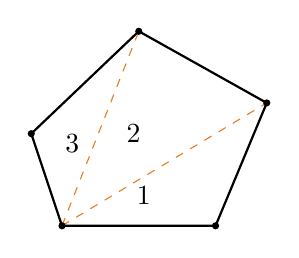
\begin{tikzpicture}[scale=1.3]
      % Pentagon triangulated
      \coordinate (A) at (0,0);
      \coordinate (B) at (1.5,0);
      \coordinate (C) at (2.0,1.2);
      \coordinate (D) at (0.75,1.9);
      \coordinate (E) at (-0.3,0.9);

      \draw[thick] (A) -- (B) -- (C) -- (D) -- (E) -- cycle;
      % Triangulate from A
      \draw[boxOrange, dashed] (A) -- (C);
      \draw[boxOrange, dashed] (A) -- (D);

      \foreach \p in {A,B,C,D,E}
        \fill (\p) circle (1pt);

      \node at (0.8,0.3) {1};
      \node at (0.7,0.9) {2};
      \node at (0.1,0.8) {3};
    \end{tikzpicture}
  \end{center}

  \begin{intuition}
    แบ่งรูป $n$ เหลี่ยมเป็นสามเหลี่ยม $n-2$ รูป (ลากจากจุดยอดหนึ่งไปทุกจุดยอดอื่น)
    แต่ละรูปมีมุมรวม $180^\circ$
  \end{intuition}

  \begin{exambox}
    $n=5$: \quad ผลรวม $= (5-2)\times 180^\circ = 540^\circ$ \quad (สามเหลี่ยม 3 รูป $\times$ $180^\circ$)
  \end{exambox}
\end{frame}

\begin{frame}{มุมภายในของรูปหลายเหลี่ยมปกติ}
  \begin{explanation}[สูตร]
    ในรูป $n$ เหลี่ยมปกติ \highlight{มุมภายในแต่ละมุม $= \dfrac{(n-2) \times 180^\circ}{n}$}
  \end{explanation}

  \begin{columns}[T]
    \column{0.4\textwidth}
      \centering
      \medskip\medskip\medskip\medskip
      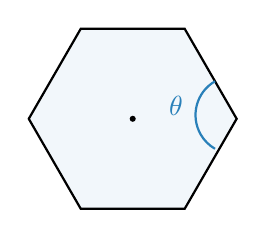
\begin{tikzpicture}[scale=1.1]
        \draw[thick, fill=boxBlue!6] (0:1.2) -- (60:1.2) -- (120:1.2) -- (180:1.2) -- (240:1.2) -- (300:1.2) -- cycle;
        \fill (0,0) circle (1pt);
        \draw[boxBlue, thick] (0.95,0.433) arc (120:240:0.45);
        \node[boxBlue] at (0.5,0.15) {$\theta$};
      \end{tikzpicture}

    \column{0.6\textwidth}
      \begin{exambox}[ตัวอย่าง]
        $n=3$: $\frac{180^\circ}{3} = 60^\circ$\quad
        $n=4$: $\frac{360^\circ}{4} = 90^\circ$\quad
      \end{exambox}

      \begin{explanation}[ผลรวมมุมภายนอก]
        \textbf{ผลรวมมุมภายนอกของรูปหลายเหลี่ยมนูนใด ๆ $= 360^\circ$}
        มุมภายนอกแต่ละมุม $= 360^\circ/n$
      \end{explanation}
  \end{columns}
\end{frame}

% ===========================================================================
%  SECTION 3: พื้นที่และเส้นรอบรูป — สามเหลี่ยม
% ===========================================================================
\section{พื้นที่และเส้นรอบรูป — สามเหลี่ยม}

\begin{frame}{สูตรพื้นที่และเส้นรอบรูปสามเหลี่ยม}
  \begin{columns}[T]
    \column{0.45\textwidth}
      \centering
      \medskip\medskip\medskip\medskip
      \medskip\medskip\medskip\medskip
      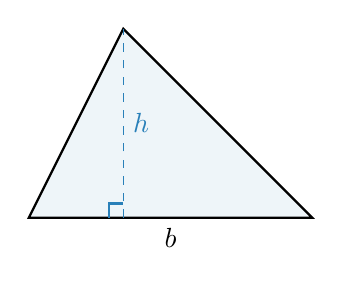
\begin{tikzpicture}[scale=1.2]
        \draw[thick, fill=boxBlue!8] (0,0) -- (3,0) node[midway, below] {$b$} -- (1,2) -- cycle;
        \draw[boxBlue, dashed] (1,0) -- (1,2) node[midway, right] {$h$};
        \draw[boxBlue, thick] (0.85,0) -- (0.85,0.15) -- (1,0.15);
      \end{tikzpicture}
      \quad $A = \dfrac{1}{2}bh$

    \column{0.55\textwidth}
      \begin{explanation}[สูตรพื้นที่]
        \begin{itemize}
          \item \textbf{พื้นฐาน}: $A = \frac{1}{2} \times \text{ฐาน} \times \text{สูง}$
          \item \textbf{เฮรอน (Heron)}: $A = \sqrt{s(s-a)(s-b)(s-c)}$
          \par \quad โดย $s = \frac{a+b+c}{2}$ (ครึ่งหนึ่งของเส้นรอบรูป)
          \item \textbf{ใช้มุม}: $A = \frac{1}{2}ab\sin C$
        \end{itemize}
      \end{explanation}

      \begin{exambox}[เส้นรอบรูป]
        $P = a + b + c$
      \end{exambox}
  \end{columns}
\end{frame}

\begin{frame}{ตัวอย่าง: พื้นที่สามเหลี่ยม}
  \begin{exambox}[โจทย์]
    สามเหลี่ยมด้านเท่ายาวด้านละ 6 ซม. จงหาพื้นที่
  \end{exambox}

  \begin{solbox}[วิธีทำ]
    \textbf{วิธีที่ 1:} $\frac{1}{2}bh$
    \begin{itemize}
      \item ความสูง $h = \sqrt{6^2 - 3^2} = \sqrt{27} = 3\sqrt{3}$
      \item $A = \frac{1}{2} \times 6 \times 3\sqrt{3} = 9\sqrt{3}$ ตร.ซม.
    \end{itemize}

    \medskip
    \textbf{วิธีที่ 2:} Heron ($s = 9$)
    \begin{itemize}
      \item $A = \sqrt{9(9-6)(9-6)(9-6)} = \sqrt{9 \times 3 \times 3 \times 3} = \sqrt{243} = 9\sqrt{3}$ ตร.ซม.
    \end{itemize}
  \end{solbox}
\end{frame}

% ===========================================================================
%  SECTION 4: พื้นที่และเส้นรอบรูป — สี่เหลี่ยม
% ===========================================================================
\section{พื้นที่และเส้นรอบรูป — สี่เหลี่ยม}

\begin{frame}{สี่เหลี่ยมจัตุรัสและสี่เหลี่ยมผืนผ้า}
  \begin{columns}[T]
    \column{0.5\textwidth}
      \centering
      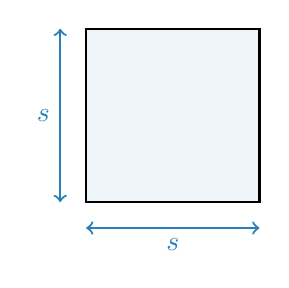
\begin{tikzpicture}[scale=1.1]
        \draw[thick, fill=boxBlue!8] (0,0) rectangle (2,2);
        \draw[boxBlue, thick, <->] (-0.3,0) -- (-0.3,2) node[midway, left] {$s$};
        \draw[boxBlue, thick, <->] (0,-0.3) -- (2,-0.3) node[midway, below] {$s$};
      \end{tikzpicture}

      \textbf{สี่เหลี่ยมจัตุรัส (Square)}

      $P = 4s$ \qquad $A = s^2$

      เส้นทแยงมุม $= s\sqrt{2}$

    \column{0.5\textwidth}
      \centering
      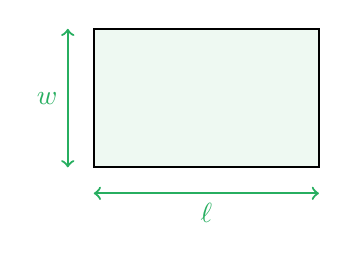
\begin{tikzpicture}[scale=1.1]
        \draw[thick, fill=boxGreen!8] (0,0) rectangle (2.6,1.6);
        \draw[boxGreen, thick, <->] (-0.3,0) -- (-0.3,1.6) node[midway, left] {$w$};
        \draw[boxGreen, thick, <->] (0,-0.3) -- (2.6,-0.3) node[midway, below] {$\ell$};
      \end{tikzpicture}

      \textbf{สี่เหลี่ยมผืนผ้า (Rectangle)}

      $P = 2(\ell + w)$ \qquad $A = \ell w$

      เส้นทแยงมุม $= \sqrt{\ell^2 + w^2}$
  \end{columns}
\end{frame}

\begin{frame}{สี่เหลี่ยมด้านขนานและสี่เหลี่ยมขนมเปียกปูน}
  \begin{columns}[T]
    \column{0.5\textwidth}
      \centering
      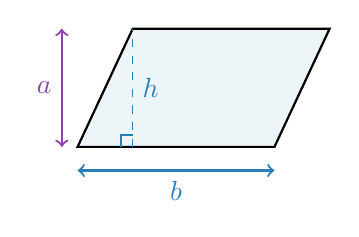
\begin{tikzpicture}[scale=1.0]
        \draw[thick, fill=boxBlue!8] (0,0) -- (2.5,0) -- (3.2,1.5) -- (0.7,1.5) -- cycle;
        \draw[boxBlue, thick, <->] (0,-0.3) -- (2.5,-0.3) node[midway, below] {$b$};
        \draw[boxBlue, dashed] (0.7,0) -- (0.7,1.5) node[midway, right] {$h$};
        \draw[boxBlue, thick] (0.55,0) -- (0.55,0.15) -- (0.7,0.15);
        \draw[boxPurple, thick, <->] (-0.2,0) -- (-0.2,1.5) node[midway, left] {$a$};
      \end{tikzpicture}

      \textbf{ด้านขนาน (Parallelogram)}

      $P = 2(a + b)$ \qquad $A = bh$

    \column{0.5\textwidth}
      \centering
      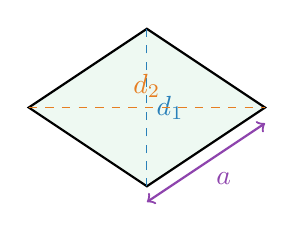
\begin{tikzpicture}[scale=1.0]
        \draw[thick, fill=boxGreen!8] (1.5,0) -- (3,1) -- (1.5,2) -- (0,1) -- cycle;
        \draw[boxBlue, dashed] (1.5,0) -- (1.5,2) node[midway, right] {$d_1$};
        \draw[boxOrange, dashed] (0,1) -- (3,1) node[midway, above] {$d_2$};
        \draw[boxPurple, thick, <->] (1.5,-0.2) -- (3,0.8) node[midway, below right] {$a$};
      \end{tikzpicture}

      \textbf{ขนมเปียกปูน (Rhombus)}

      $P = 4a$ \qquad $A = \frac{1}{2}d_1 d_2 = ah$
  \end{columns}
\end{frame}

\begin{frame}{สี่เหลี่ยมคางหมูและสี่เหลี่ยมรูปว่าว}
  \begin{columns}[T]
    \column{0.5\textwidth}
      \centering
      \begin{tikzpicture}[scale=1.0]
        \draw[thick, fill=boxBlue!8] (0,0) -- (3,0) -- (2.4,1.5) -- (0.4,1.5) -- cycle;
        \draw[boxBlue, thick, <->] (0,-0.3) -- (3,-0.3) node[midway, below] {$a$ (ฐานคู่ขนาน)};
        \draw[boxOrange, thick, <->] (0.4,1.8) -- (2.4,1.8) node[midway, above] {$b$};
        \draw[boxBlue, dashed] (1.5,0) -- (1.5,1.5) node[midway, right] {$h$};
        \draw[boxBlue, thick] (1.35,0.1) -- (1.35,0.25) -- (1.5,0.25);
      \end{tikzpicture}

      \textbf{คางหมู (Trapezoid)}

      $A = \dfrac{1}{2}(a+b)h$

      $P =$ ผลรวมของ 4 ด้าน

    \column{0.5\textwidth}
      \centering
      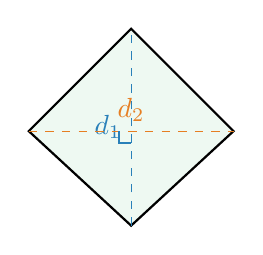
\begin{tikzpicture}[scale=1.0]
        \draw[thick, fill=boxGreen!8] (1.5,0) -- (2.8,1.2) -- (1.5,2.5) -- (0.2,1.2) -- cycle;
        \draw[boxBlue, dashed] (1.5,0) -- (1.5,2.5) node[midway, left] {$d_1$};
        \draw[boxOrange, dashed] (0.2,1.2) -- (2.8,1.2) node[midway, above] {$d_2$};
        % Right angle marker
        \draw[boxBlue, thick] (1.5,1.05) -- (1.35,1.05) -- (1.35,1.2);
      \end{tikzpicture}

      \textbf{รูปว่าว (Kite)}

      $A = \dfrac{1}{2}d_1 d_2$

      $P = 2(a+b)$ \quad ($a,b$ = ด้านคู่ที่เท่ากัน)
  \end{columns}
\end{frame}

\begin{frame}{สรุปสูตรพื้นที่สี่เหลี่ยม}
  \begin{center}
    \renewcommand{\arraystretch}{1.2}
    \begin{tabular}{l|c|c}
      \textbf{รูป} & \textbf{พื้นที่ ($A$)} & \textbf{เส้นรอบรูป ($P$)} \\
      \hline
      จัตุรัส & $s^2$ & $4s$ \\
      ผืนผ้า & $\ell w$ & $2(\ell + w)$ \\
      ด้านขนาน & $bh$ & $2(a+b)$ \\
      ขนมเปียกปูน & $\frac{1}{2}d_1d_2$ หรือ $ah$ & $4a$ \\
      คางหมู & $\frac{1}{2}(a+b)h$ & ผลรวม 4 ด้าน \\
      รูปว่าว & $\frac{1}{2}d_1d_2$ & $2(a+b)$ \\
    \end{tabular}
  \end{center}

  \begin{intuition}[สังเกต!]
    ขนมเปียกปูนกับรูปว่าวใช้ $\frac{1}{2}d_1d_2$ เหมือนกัน \quad $|$ \quad
    จัตุรัสคือกรณีพิเศษของผืนผ้า ($\ell = w = s$)
  \end{intuition}
\end{frame}

% ===========================================================================
%  SECTION 5: วงกลม
% ===========================================================================
\section{วงกลม (Circle)}

\begin{frame}{สูตรวงกลม}
  \begin{columns}[T]
    \column{0.5\textwidth}
      \centering
      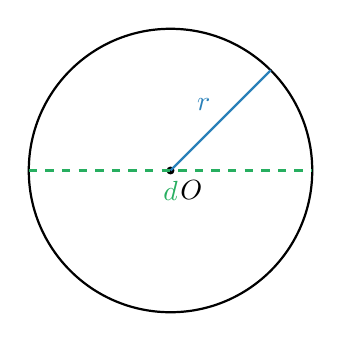
\begin{tikzpicture}[scale=1.2]
        \draw[thick] (0,0) circle (1.5);
        \fill (0,0) circle (1.2pt) node[below right] {$O$};
        \draw[boxBlue, thick] (0,0) -- (1.061,1.061) node[midway, above left] {$r$};
        \draw[boxGreen, thick, dashed] (-1.5,0) -- (1.5,0) node[midway, below] {$d$};
      \end{tikzpicture}

    \column{0.5\textwidth}
      \begin{explanation}[สูตร]
        \begin{itemize}
          \item \textbf{เส้นรอบวง}: $C = 2\pi r = \pi d$
          \item \textbf{พื้นที่}: $A = \pi r^2$
          \item \textbf{ส่วนโค้ง} (มุม $\theta^\circ$): $L = \frac{\theta}{360} \times 2\pi r$
          \item \textbf{เซกเตอร์}: $A = \frac{\theta}{360} \times \pi r^2$
          \item \textbf{เซกเมนต์}: $A_{\text{sec}} - A_{\triangle}$
        \end{itemize}
      \end{explanation}
  \end{columns}

  \begin{exambox}[ตัวอย่าง]
    $r = 7$ ซม., $\pi \approx \frac{22}{7}$ \quad $\rightarrow$ \quad $C = 44$ ซม., $A = 154$ ตร.ซม.
  \end{exambox}
\end{frame}

% ===========================================================================
%  SECTION 6: รูปหลายเหลี่ยมปกติ
% ===========================================================================
\section{พื้นที่รูปหลายเหลี่ยมปกติ}

\begin{frame}{พื้นที่รูปหลายเหลี่ยมปกติ}
  \begin{explanation}[สูตร]
    \highlight{$A = \frac{1}{2} P a$} \quad โดย $P =$ เส้นรอบรูป, $a =$ \textbf{ระยะแนบใน (apothem)}
     ระยะตั้งฉากจากจุดศูนย์กลางไปยังด้าน
  \end{explanation}

  \begin{center}
    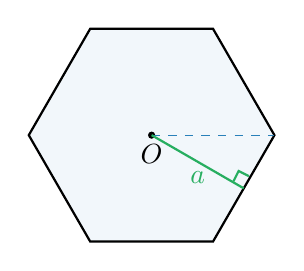
\begin{tikzpicture}[scale=1.3]
      % Regular hexagon with apothem
      \draw[thick, fill=boxBlue!6] (0:1.2) -- (60:1.2) -- (120:1.2) -- (180:1.2) -- (240:1.2) -- (300:1.2) -- cycle;
      \fill (0,0) circle (1pt) node[below] {$O$};

      % Apothem to one side
      \draw[boxBlue, dashed] (0,0) -- (0:1.2);
      % \draw[boxOrange, thick] (0,0) -- (0.6,0) node[midway, above] {$r$};

      % Apothem to bottom-right side: side from 300° to 0°
      % Side midpoint at angle -30° from center
      \draw[boxGreen, thick] (0,0) -- (-30:1.039) node[midway, below] {$a$};
      \draw[boxGreen, thick] (0.8,-0.45) -- (0.85,-0.35) -- (0.95,-0.4);
    \end{tikzpicture}
  \end{center}

  \begin{exambox}[ตัวอย่าง: หกเหลี่ยมปกติด้านละ 6]
    $P = 6 \times 6 = 36$
    \par $a = \sqrt{6^2 - 3^2} = \sqrt{27} = 3\sqrt{3}$ \quad (แบ่งเป็นสามเหลี่ยมด้านเท่า 6 รูป)
    \par $A = \frac{1}{2} \times 36 \times 3\sqrt{3} = 54\sqrt{3}$
  \end{exambox}
\end{frame}

% ===========================================================================
%  SECTION 7: ตัวอย่างโจทย์
% ===========================================================================
\section{ตัวอย่างโจทย์ประยุกต์}

\begin{frame}{ตัวอย่าง: รูปหลายเหลี่ยม}
  \begin{exambox}[โจทย์ 1]
    รูปแปดเหลี่ยมปกติมีมุมภายในกี่องศา? และมีเส้นทแยงมุมกี่เส้น?
  \end{exambox}

  \begin{solbox}[วิธีทำ]
    มุมภายใน: $\frac{(8-2) \times 180^\circ}{8} = 135^\circ$ \qquad
    เส้นทแยงมุม: $\frac{8(8-3)}{2} = 20$ เส้น
  \end{solbox}

  \begin{exambox}[โจทย์ 2]
    รูปหลายเหลี่ยมปกติรูปหนึ่งมีมุมภายใน $156^\circ$ จงหาจำนวนด้าน
  \end{exambox}

  \begin{solbox}[วิธีทำ]
    $\frac{(n-2)180^\circ}{n} = 156^\circ \;\Rightarrow\; 180n-360=156n \;\Rightarrow\; n=15$
  \end{solbox}
\end{frame}

\begin{frame}{ตัวอย่าง: พื้นที่}
  \begin{exambox}[โจทย์]
    สี่เหลี่ยมคางหมูมีด้านคู่ขนานยาว 8 และ 12 ซม. สูง 5 ซม. จงหาพื้นที่
  \end{exambox}

  \begin{solbox}[วิธีทำ]
    $A = \frac{1}{2}(8+12) \times 5 = 50$ ตร.ซม.
  \end{solbox}

  \begin{exambox}[โจทย์]
    สี่เหลี่ยมขนมเปียกปูนมีเส้นทแยงมุมยาว 10 และ 24 ซม. จงหาพื้นที่และความยาวด้าน
  \end{exambox}

  \begin{solbox}[วิธีทำ]
    $A = \frac{1}{2} \times 10 \times 24 = 120$ ตร.ซม. \quad
    $a = \sqrt{5^2 + 12^2} = 13$ ซม.
  \end{solbox}
\end{frame}

\begin{frame}{ตัวอย่าง: พื้นที่รูปหลายเหลี่ยมปกติ}
  \begin{exambox}[โจทย์]
    รูปหกเหลี่ยมปกติแนบในวงกลมรัศมี 10 ซม. จงหาพื้นที่
  \end{exambox}

  \begin{solbox}[วิธีทำ]
    แนบในวงกลม $\rightarrow$ $s = r = 10$ ซม.

    วิธี 1: $A = \frac{3\sqrt{3}}{2}s^2 = 150\sqrt{3}$ ตร.ซม.

    วิธี 2: 6 รูป $\triangle$ ด้านเท่า: $A = 6 \times \frac{\sqrt{3}}{4} \times 100 = 150\sqrt{3}$ ตร.ซม.
  \end{solbox}
\end{frame}

% ===========================================================================
%  SUMMARY
% ===========================================================================
\section{สรุป}

\begin{frame}{สรุปเนื้อหา}
  \begin{explanation}[สิ่งที่ได้เรียนรู้]
    \begin{enumerate}
      \item \textbf{รูปหลายเหลี่ยม}: นูน (ทุกมุม $< 180^\circ$) / เว้า (มีมุมกลับ), ปกติ (ด้านเท่า, มุมเท่า)
      \item \textbf{เส้นทแยงมุม}: $\frac{n(n-3)}{2}$ เส้น
      \item \textbf{มุมภายใน}: ผลรวม $= (n-2) \times 180^\circ$,
             ปกติแต่ละมุม $= \frac{(n-2) \times 180^\circ}{n}$
      \item \textbf{มุมภายนอก}: ผลรวม $= 360^\circ$ เสมอ
      \item \textbf{พื้นที่สามเหลี่ยม}: $\frac{1}{2}bh$, $\sqrt{s(s-a)(s-b)(s-c)}$, $\frac{1}{2}ab\sin C$
      \item \textbf{พื้นที่สี่เหลี่ยม}: จัตุรัส $s^2$, ผืนผ้า $\ell w$, ด้านขนาน $bh$,
             ขนมเปียกปูน $\frac{1}{2}d_1d_2$, คางหมู $\frac{1}{2}(a+b)h$, รูปว่าว $\frac{1}{2}d_1d_2$
      \item \textbf{วงกลม}: $C = 2\pi r$, $A = \pi r^2$
      \item \textbf{รูปหลายเหลี่ยมปกติ}: $A = \frac{1}{2}Pa$
    \end{enumerate}
  \end{explanation}
\end{frame}

\end{document}
